\documentclass[paper=a4, fontsize=11pt]{scrartcl}
\usepackage[letterpaper, margin=0.85in]{geometry}
\usepackage[T1]{fontenc}
\usepackage{fourier}
\usepackage{ragged2e}

\usepackage[english]{babel}															
\usepackage[protrusion=true,expansion=true]{microtype}	
\usepackage{amsmath,amsfonts,amsthm} 
\usepackage[pdftex]{graphicx}	
\usepackage{url}


\usepackage{sectsty}
\allsectionsfont{\centering \normalfont\scshape}

% Libraries added by Kyle
\usepackage[parfill]{parskip} % Skip in between paragraphs instead of indenting
\usepackage{wrapfig} % Figures to the side of text / text wrapping around figures
\usepackage{caption} % Captioning of figures
\usepackage{fancyref} % Referencing of figures and updates automatically as figures change number
% End libraries added by Kyle

\usepackage{fancyhdr}
\pagestyle{fancyplain}
\fancyhead{}											
\fancyfoot[L]{}											
\fancyfoot[C]{}											
\fancyfoot[C]{\thepage}									
\renewcommand{\headrulewidth}{0pt}			
\renewcommand{\footrulewidth}{0pt}				
\setlength{\headheight}{13.6pt}


\numberwithin{equation}{section}		
\numberwithin{figure}{section}			
\numberwithin{table}{section}				


\newcommand{\horrule}[1]{\rule{\linewidth}{#1}} 

\title{
		%\vspace{-1in} 	
		\usefont{OT1}{bch}{b}{n}
		\normalfont \normalsize \textsc{University of California, Los Angeles} \\ [25pt]
		\horrule{0.5pt} \\[0.4cm]
		\huge Cry, Cry, Cry \\
		\horrule{2pt} \\[0.5cm]
}
\author{
		\normalfont \normalsize Kyle Colton \\
        \normalfont \normalsize Christian Gao \\
        \normalfont \normalsize  Benjamin Hong \\
        \normalfont \normalsize Feiran Zhu\\
}
\date{}


\begin{document}
\maketitle


\includegraphics[width=\textwidth]{baby.jpg}
\newpage

\tableofcontents
\newpage
\noindent \horrule{0.5pt} 
{\textbf{\\ Objective.}}
The purpose of this study is to discuss algorithms designed to predict whether or not a baby is crying. 
{\textbf{\\ Data Collection and Procedure.}}
We were given a multitude of audio files (in WAV format) of animal, baby, and adult sounds. We analyzed the pitch of each sound using two different procedures: (1) using FOSS \textit{aubio} and conducting K-means clustering, which is an iterative classification method that we will discuss in more detail later, and support vector machine (SVM) classification and (2) using a specially designed pitch extraction algorithm to ultimately use the Baum-Welch algorithm to answer a number of questions that we will make clear throughout the report.
{\textbf{\\ Conclusion.}}
We arrived at a decent classification algorithm using K-means and SVM, but because of limitations in the data, we did not end up with an extremely successful algorithm based on HMM.  \\
\horrule{0.5pt} \\[0.4cm]
% * <bendhong@ucla.edu> 2015-06-06T23:36:04.154Z:
%
% 
%
% * <bendhong@ucla.edu> 2015-06-06T23:36:05.493Z:
%
% 
%
\section{Abstract}
% * <bendhong@ucla.edu> 2015-06-06T23:36:06.752Z:
%
% 
%
Caring for a baby requires patience and effective communication. A caretaker attends to the baby when he/she cries, but this strictly involves an auditory process. We can see how this becomes problematic for parents who are deaf or have difficulty hearing. Fortunately, because of technological advances, there are now devices that assist parents in determining whether or not their child is crying. Of course, for a device to accurately decipher noises, the algorithm must be able to distinguish between different noises (e.g., between a dog crying and a baby crying). This report discusses the algorithms we designed to predict the baby's emotional state---that is, is the baby crying, laughing, or neutral? 


\section{Questions}
\begin{enumerate}
	\item Can we design an algorithm that accurately predicts whether or not a baby is crying?
	\item Given that our algorithm works, what is its prediction rate---that is, how often does our algorithm successfully classify noises into their respective categories?
\end{enumerate}

\section{Variable Description}

\section{Statistical Methods Used}
\subsection{Hidden Markov Model}
\begin{center}
\begin{tabular}{ |c|c|c|c| } 
 \hline
       & Cry & Neutral & Laugh \\
 \hline
 Cry & 0.8 & 0.15 & 0.05 \\ 
 Neutral & 0.2 & 0.6 & 0.2 \\ 
 Laugh & 0.05 & 0.35 & 0.6 \\
 \hline
\end{tabular}
\end{center}

\centering $\downarrow$

\begin{center}
\begin{tabular}{ |c|c|c|c| } 
 \hline
       & Cry & Neutral & Laugh \\
 \hline
 Cry & 0.85 & 0.1 & 0.05 \\ 
 Neutral & 0.15 & 0.7 & 0.15 \\ 
 Laugh & 0.1 & 0.4 & 0.5 \\
 \hline
\end{tabular}
\end{center}

\justifying Let $X_t$ be a discrete hidden random variable with $N$ possible values. $P(X_t|X_{t-1})$ is independent of time $t$, so our transition matrix will be:

\begin{equation}
A = \{a_{ij}\} = P(X_t = j|X_{t-1} = i)
\end{equation}

\noindent \\ The initial state distribution at, for example, $t = 1$, is given by: $\boxed{\pi_i = P(X_1 = i)}$ \\

\noindent The probability of a certain observation occurring at time $t$ for state $j$ is given by: $\boxed{b_j(y_t) = P(Y_t = y_t|X_t = j)}$ \\

\noindent The observation sequence should look like $Y = (Y_1 = y_1, Y_2 = y_2, \ldots, Y_t = y_t)$

\noindent Altogether, we now have a hidden Markov chain that can be described by:

\begin{equation}
\boxed{\theta = (A, B, \pi)}
\end{equation}

\section{Summary of Findings}
\section{Classification using Pitch Analysis}
Pitch detection and analysis was explored as a method to identify baby cries. The detection method relies on the assumption that pitch patterns for each sound type will differ, but within the sound types each sample will be similar.

\begin{wrapfigure}{r}{.4\textwidth}
\begin{center}
\vspace{-20pt}
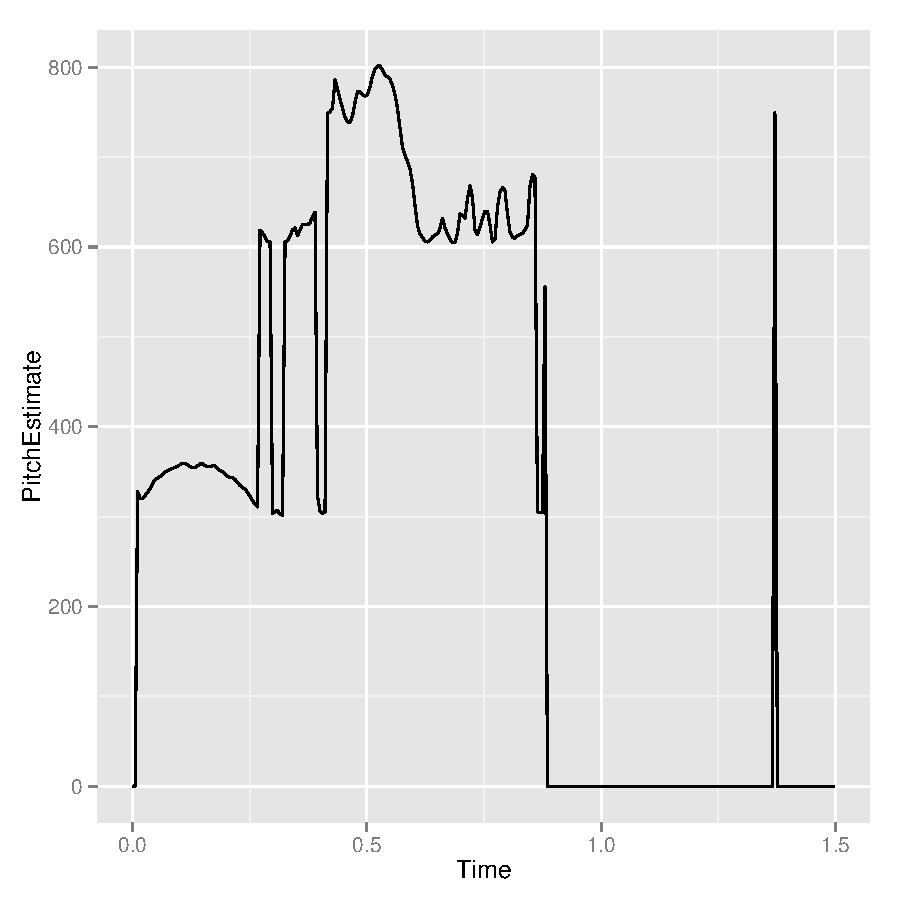
\includegraphics[width=.38\textwidth]{pitch_time.pdf}
\caption{Pitch estimate of a \texttt{wav} file}\label{fig:aubiograph}
\vspace{-20pt}
\end{center}
\end{wrapfigure}

\noindent Raw audio files (stored as \texttt{wav}) were run through a Free/Libre and Open Source Software package called Aubio\footnote{Package information can be found at \url{aubio.org} or at http://git.aubio.org}. Aubio is a C-based audio labeling tool that includes several methods and controllable methods for pitch detection in an audio stream.

\noindent In order to complete pitch analysis, each 1.5 second \texttt{wav} file was fed through Aubio to get time-series pitch data, then broken into ``events'' based on silence. In figure \ref{fig:aubiograph}, we see an estimate of pitches over time for one such file. This file, for example would be broken into two events. The main event stretches from approximately $t=0.00$ to $t=0.85$. A second event occurs around $t=1.40$.

\noindent Looking at the graph, it appears that the second event in this file is an error. It is a blip caused by something in the recording that we can safely ignore if we can identify it and separate it from the good data. An easy approximation is to ignore all events shorter than a set time interval. After testing all time intervals using a given model, $t=0.1$ seconds was chosen as the cutoff for ``real'' versus ``fake'' events.

\begin{wrapfigure}{l}{.3\textwidth}
\begin{center}
\vspace{-15pt}
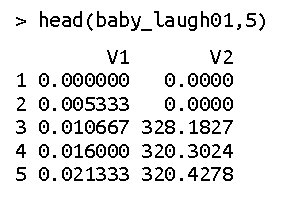
\includegraphics[width=.28\textwidth]{aubio_out.pdf}
\caption{Data from Aubio with time (l) and pitch estimate (r)}\label{fig:headaubio}
\end{center}
\vspace{-20pt}
\end{wrapfigure}

\noindent After events were detected and pre-processed, summary statistics were collected on each event. Each event was stored with filename, event type (baby\_cry, baby\_laugh, etc.), minimum pitch, 1st quartile, median pitch, 3rd quartile, maximum pitch, mean pitch, and length of the event. Models were then run on these summary statistics to capture and classify them and compare them to the originating source. To start with, the models were built around using the events individually. Eventually, smarter models were built to consider all events from a single file as a unit and decide by voting on the predicted classification of those files.


\subsection{K-Means Applied to Pitch Estimates}
\subsubsection{Performance of K-Means}
\subsection{Support Vector Machine Applied to Pitch Estimates}
\subsubsection{Performance of SVM}

\subsection{Using Baum-Welch Algorithm}

\section{Conclusion}

\section{Shortcomings}

\section{Recommendations}

\end{document}